% 计算方法实验报告：数值积分算法的比较实现
% 编译：XeLaTeX（中文必须 XeLaTeX），在 docs/ 目录下执行两遍 xelatex 以生成目录。
\documentclass[12pt,a4paper]{ctexart}
% 中文默认使用 ctex 自带的 fandol 字体（TeX Live / MiKTeX 均自带）。
% 若在 Windows 上希望使用宋体/黑体，可改为 fontset=windows。

\usepackage{amsmath,amssymb}
\usepackage{graphicx}
\usepackage{booktabs}
\usepackage{geometry}
\usepackage{caption}
\usepackage{listings}
\usepackage{xcolor}
\usepackage{tcolorbox}
\usepackage{float}   % 用 [H] 精确放置图表，避免浮动造成的大片空白
\usepackage{hyperref}
\hypersetup{hidelinks}

\geometry{left=2.6cm,right=2.6cm,top=2.6cm,bottom=2.6cm}
\emergencystretch=1.5em   % 中文不能断词，留一点兜底伸缩，避免行末溢出
\graphicspath{{assets/}}
\captionsetup{font=small,labelsep=quad}
\renewcommand{\arraystretch}{1.15}

% ---------------------------------------------------------------
% 代码排版：仿 VS Code Dark+ 配色，等宽字体用 JetBrains Mono（缺失时回退 DejaVu Sans Mono）。
% XeLaTeX 下 listings 会把非 ASCII 字符交给 xeCJK 处理，中文注释走 \CJKmonofont，无需 escape。
\usepackage{fontspec}
\IfFontExistsTF{JetBrainsMono Nerd Font}
    {\setmonofont{JetBrainsMono Nerd Font}[Scale=0.80]}
    {\setmonofont{DejaVu Sans Mono}[Scale=0.86]}
\IfFontExistsTF{Noto Sans CJK SC}
    {\setCJKmonofont{Noto Sans CJK SC}[Scale=0.86]}
    {\setCJKmonofont{FandolHei}[Scale=0.86]}

\definecolor{codebg}{HTML}{1E1E1E}   % 编辑器背景
\definecolor{codefg}{HTML}{D4D4D4}   % 前景
\definecolor{codekw}{HTML}{569CD6}   % 关键字：蓝
\definecolor{codestr}{HTML}{CE9178}  % 字符串：橙
\definecolor{codecmt}{HTML}{6A9955}  % 注释：绿

\lstdefinestyle{vscode}{
    language=Python,
    deletekeywords=[2]{str},   % 内置类型名不算关键字，与 VS Code 一致
    basicstyle=\ttfamily\footnotesize\color{codefg},
    keywordstyle=\color{codekw},
    stringstyle=\color{codestr},
    commentstyle=\color{codecmt},
    moredelim=**[s][\color{codestr}]{"""}{"""},   % docstring 按字符串着色
    moredelim=**[s][\color{codestr}]{'''}{'''},
    backgroundcolor=\color{codebg},
    columns=fullflexible,
    keepspaces=true,
    showstringspaces=false,
    upquote=true,              % 直引号 " ' 而不是弯引号
    breaklines=true,
    breakindent=2em,
    tabsize=4,
    numbers=left,              % 沿用源码真实行号，中灰，在深底上可见但不抢眼
    numberstyle=\tiny\color{codefg!55},
    numbersep=1.0em,
    xleftmargin=2.2em,
    xrightmargin=0pt,
    aboveskip=0pt,
    belowskip=0pt,
}

% 代码块外壳：深色圆角框，行号与代码都在框内（同 VS Code 观感）
\newtcolorbox{codebox}{
    colback=codebg, colframe=codebg, boxrule=0pt, arc=2pt,
    left=0.6em, right=0.6em, top=0.5em, bottom=0.5em,
    before skip=0.9em, after skip=0.9em,
}
\lstset{style=vscode}

% 行内代码：同样的深色小底块
\newcommand{\code}[1]{%
    {\colorbox{codebg}{\color{codefg}\ttfamily\CJKfamily{tt}\footnotesize\ #1\ }}}%
\setlength{\fboxsep}{1.6pt}

% 源码在上一级目录。\src{文件}{起}{止} 只贴关键片段，行号沿用源码真实行号。
\newcommand{\src}[3]{%
    \begin{codebox}%
    \lstinputlisting[style=vscode,linerange={#2-#3},firstnumber=#2]{../#1}%
    \end{codebox}}

% 放宽浮动体限制
\renewcommand{\topfraction}{0.92}
\renewcommand{\bottomfraction}{0.85}
\renewcommand{\textfraction}{0.08}
\renewcommand{\floatpagefraction}{0.7}
\setcounter{topnumber}{3}
\setcounter{bottomnumber}{3}
\setcounter{totalnumber}{4}

\begin{document}

% ==================== 封面 ====================
\begin{titlepage}
    \centering
    \vspace*{1.6cm}
    
\includegraphics[width=4.2cm]{assets/logo.png}\\[1.2cm]
    {\zihao{2} \textbf{汕头大学}}\\[0.6cm]
    {\zihao{1} \textbf{计 算 方 法 实 验 报 告}}\\[2cm]
    {\zihao{3} 实验二：数值积分算法的比较实现}\\[2.4cm]

    \zihao{4}
    \renewcommand{\arraystretch}{1.8}
    \begin{tabular}{rl}
        姓\hspace{2em}名： & 黄应辉 \\
        学\hspace{2em}号： & 2024611031 \\
        专\hspace{2em}业： & 计算机科学与技术 \\
        指导教师： & 陈夏铭\\
    \end{tabular}

    \vfill
    {\zihao{4} \the\year 年 11 月 24 日}
\end{titlepage}

% ==================== 目录 ====================
\tableofcontents
\newpage

% ==================== 正文 ====================
% ---------------------------------------------------------------
\section{被积函数与真值}\label{sec:function}

本次实验计算积分
\begin{equation}
    I=\int_0^1\frac{\sin x}{x}\,\mathrm{d}x .
    \label{eq:target}
\end{equation}
$f(x)=\sin x/x$ 在 $x=0$ 处没有定义，但极限 $\lim_{x\to0}f(x)=1$ 存在，是可去奇点，
补定义 $f(0)=1$ 后它在 $[0,1]$ 上处处光滑；而它的原函数不是初等函数，
因此式 \eqref{eq:target} 没有闭式的解析结果，只能数值估算。该积分就是正弦积分在 1 处的值 $\mathrm{Si}(1)$。

为了给各算法的误差提供基准，把 $\sin x$ 展成幂级数再逐项积分：
\begin{equation}
    \frac{\sin x}{x}=\sum_{k=0}^{\infty}\frac{(-1)^k x^{2k}}{(2k+1)!}
    \quad\Longrightarrow\quad
    I=\mathrm{Si}(1)=\sum_{k=0}^{\infty}\frac{(-1)^k}{(2k+1)\,(2k+1)!}
    \label{eq:series}
\end{equation}
\begin{equation}
    I=0.946083\,070367\,183014\,9413\cdots
    \label{eq:exact}
\end{equation}
通项以阶乘速度衰减，取 12 项即可在双精度下精确。
后文的“误差”均指 $|I_{\text{近似}}-I|$，其中 $I$ 取式 \eqref{eq:exact}。

所有算法都只依赖“给 $x$ 返回 $f(x)$”这一接口，所以先把被积函数、积分区间与真值集中在一处（\code{function.py}），
算法模块只接收 \code{f, a, b} 作参数，不绑定具体问题。
\src{function.py}{21}{38}
\src{function.py}{41}{56}

\code{f} 在 $x=0$ 处直接返回 1，避免 0/0——梯形、辛普森都会在端点 $a=0$ 求值。
\code{si1} 按式 \eqref{eq:series} 取 12 项，模块加载时算一次存入 \code{EXACT}，之后所有误差都相对它计算。

% ---------------------------------------------------------------
\section{五种求积方法}\label{sec:methods}

五种方法按“用多少个函数值、拟合得多精”的顺序展开：矩形 → 梯形 → 辛普森属于\textbf{牛顿-柯特斯}家族，
节点等距、权重固定，精度靠加密区间提升；龙贝格与高斯则从两个方向突破：前者对梯形结果做\textbf{外推}，
后者把\textbf{节点位置}也作为自由度。每种方法一个模块，统一提供计算近似值的 \code{xxx\_rule(f, a, b, ...)}、
给出求值次数的 \code{evaluations(...)} 和画近似图形的 \code{draw(...)}，由 \code{main.py} 以相同方式调用。

\begin{figure}[H]
    \centering
    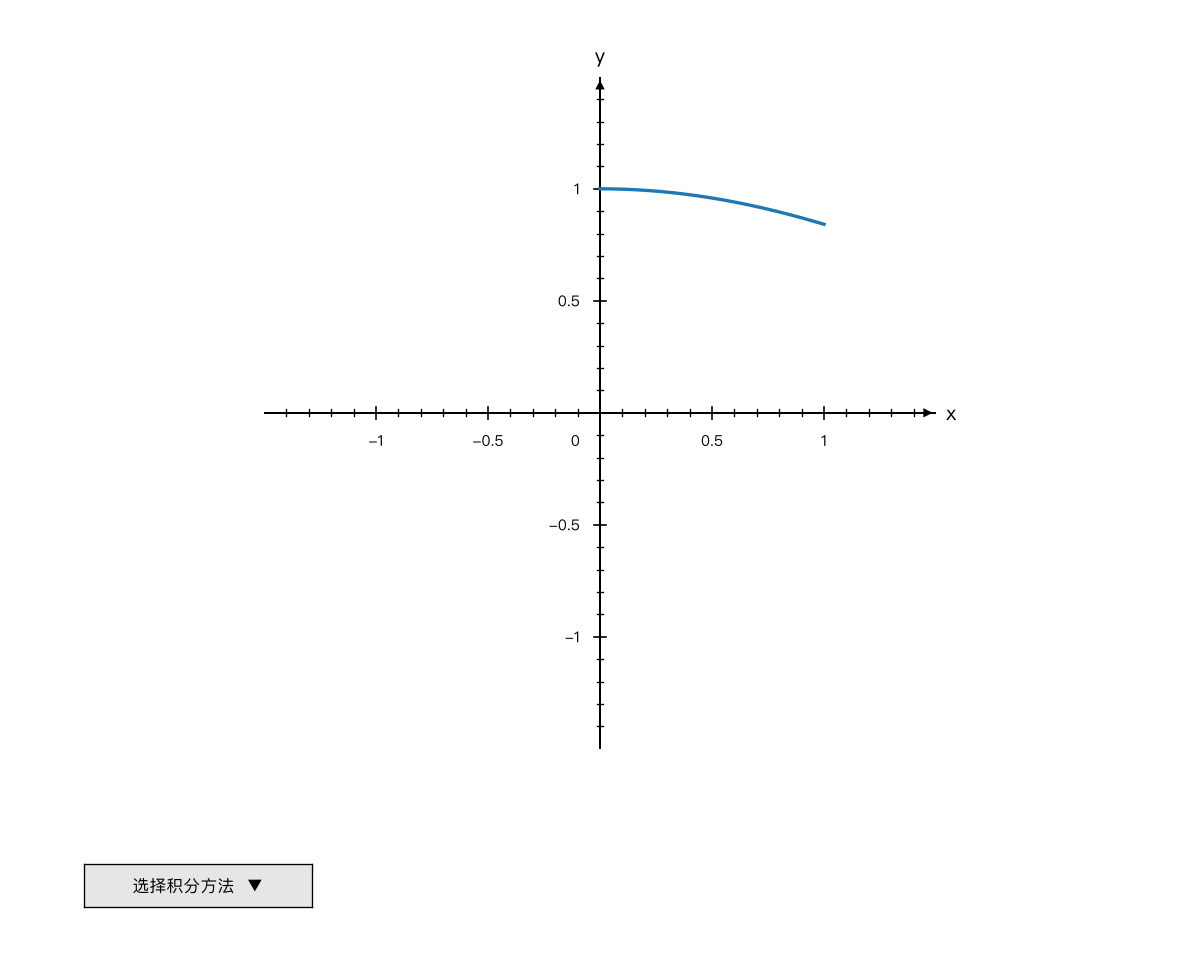
\includegraphics[width=0.48\textwidth]{ui_default.png}
    \caption{程序初始界面：只显示被积函数与下拉栏}
    \label{fig:default}
\end{figure}

程序用 \code{uv run main.py} 启动，在下拉栏中选择方法、拖动滑块调参数，
下方信息栏显示近似值、真值、误差与函数求值次数（图 \ref{fig:default}）。

% ---------------------------------------------------------------
\subsection{矩形法}\label{subsec:rectangle}

把 $[a,b]$ 等分为 $n$ 段，步长 $h=(b-a)/n$，每段用一个函数值作高、$h$ 作宽得到矩形，求和即近似值：
\begin{equation}
    R_n=h\sum_{k=0}^{n-1}f(x_k^{*}),\qquad
    x_k^{*}=a+kh,\;\;a+\left(k+\tfrac12\right)h,\;\;a+(k+1)h,
    \label{eq:rect}
\end{equation}
分别对应左、中、右三种取法。左、右矩形误差 $O(h)$，中矩形 $O(h^2)$。
实现时三种取法只差“第 $k$ 段在哪取函数值”，封装在 \code{sample\_x} 一个函数里：
\src{rectangle.py}{25}{35}
\code{pieces} 据此生成每段的 \code{(左端, 宽, 高)}，计算与画图共用同一份数据：
\src{rectangle.py}{38}{50}
\code{draw} 用这份数据画 $n$ 个矩形并标出取样点，运行效果如图 \ref{fig:rectangle}。

\begin{figure}[H]
    \centering
    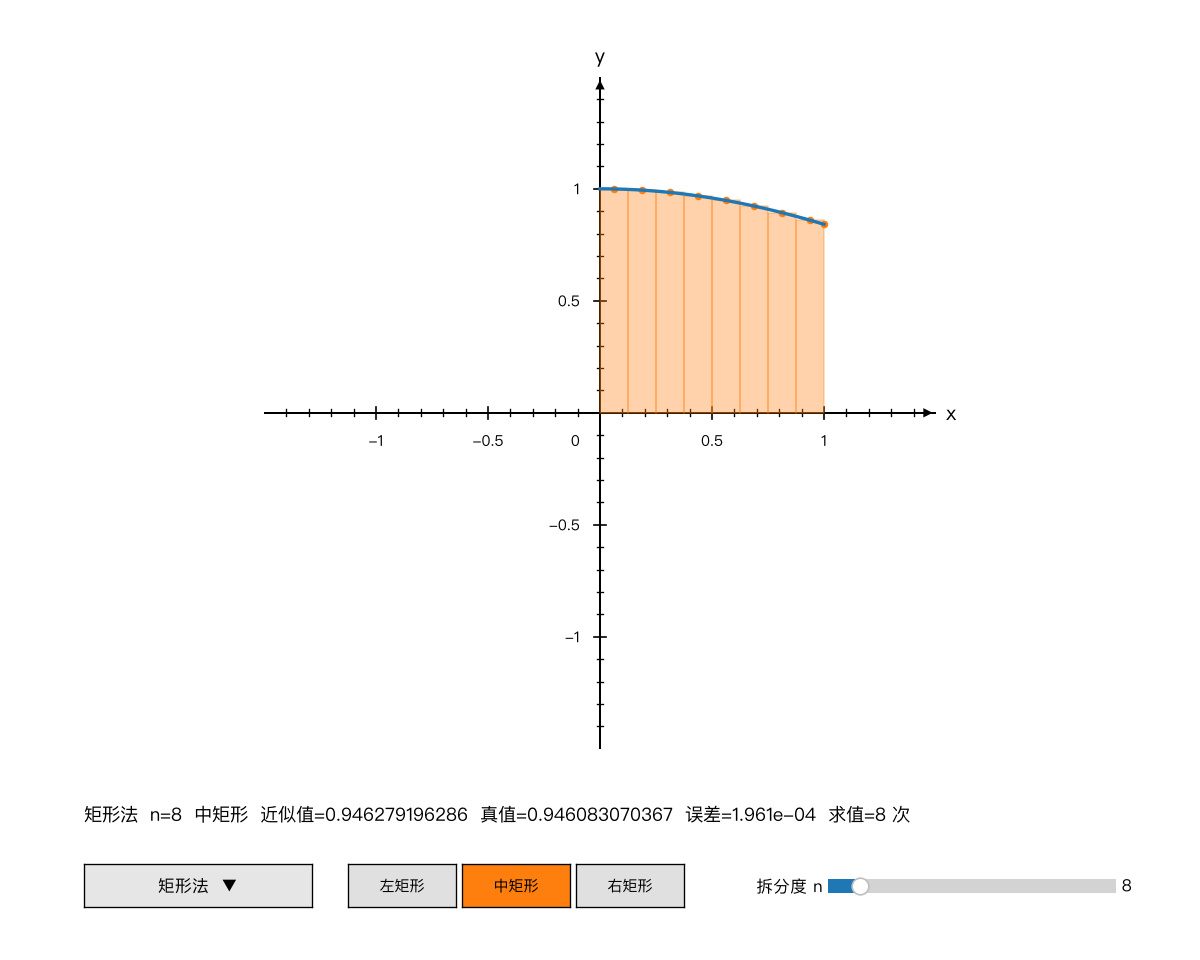
\includegraphics[width=0.48\textwidth]{ui_rectangle.png}
    \caption{矩形法（中矩形，$n=8$）：误差 $1.96\times10^{-4}$，8 次求值}
    \label{fig:rectangle}
\end{figure}

$n=8$ 时中矩形得 $R_8=0.946279196286$，误差 $1.96\times10^{-4}$，共 8 次函数求值。

% ---------------------------------------------------------------
\subsection{梯形法}\label{subsec:trapezoid}

每段用过两端点的弦代替曲线，得梯形面积 $\frac{h}{2}[f(x_k)+f(x_{k+1})]$；相邻梯形在公共节点处的高度被算了两次，
合并后即复化梯形公式
\begin{equation}
    T_n=\frac{h}{2}\left[f(a)+2\sum_{k=1}^{n-1}f(a+kh)+f(b)\right],\qquad h=\frac{b-a}{n}.
    \label{eq:trap}
\end{equation}
误差 $O(h^2)$。按式 \eqref{eq:trap} 累加：先放两端点，内部节点乘 2，最后统一乘 $h/2$，每个节点只求一次函数值：
\src{trapezoid.py}{21}{36}

运行效果如图 \ref{fig:trapezoid}，$n=8$ 时 $T_8=0.945690863583$，误差 $3.92\times10^{-4}$，共 9 次函数求值。

\begin{figure}[H]
    \centering
    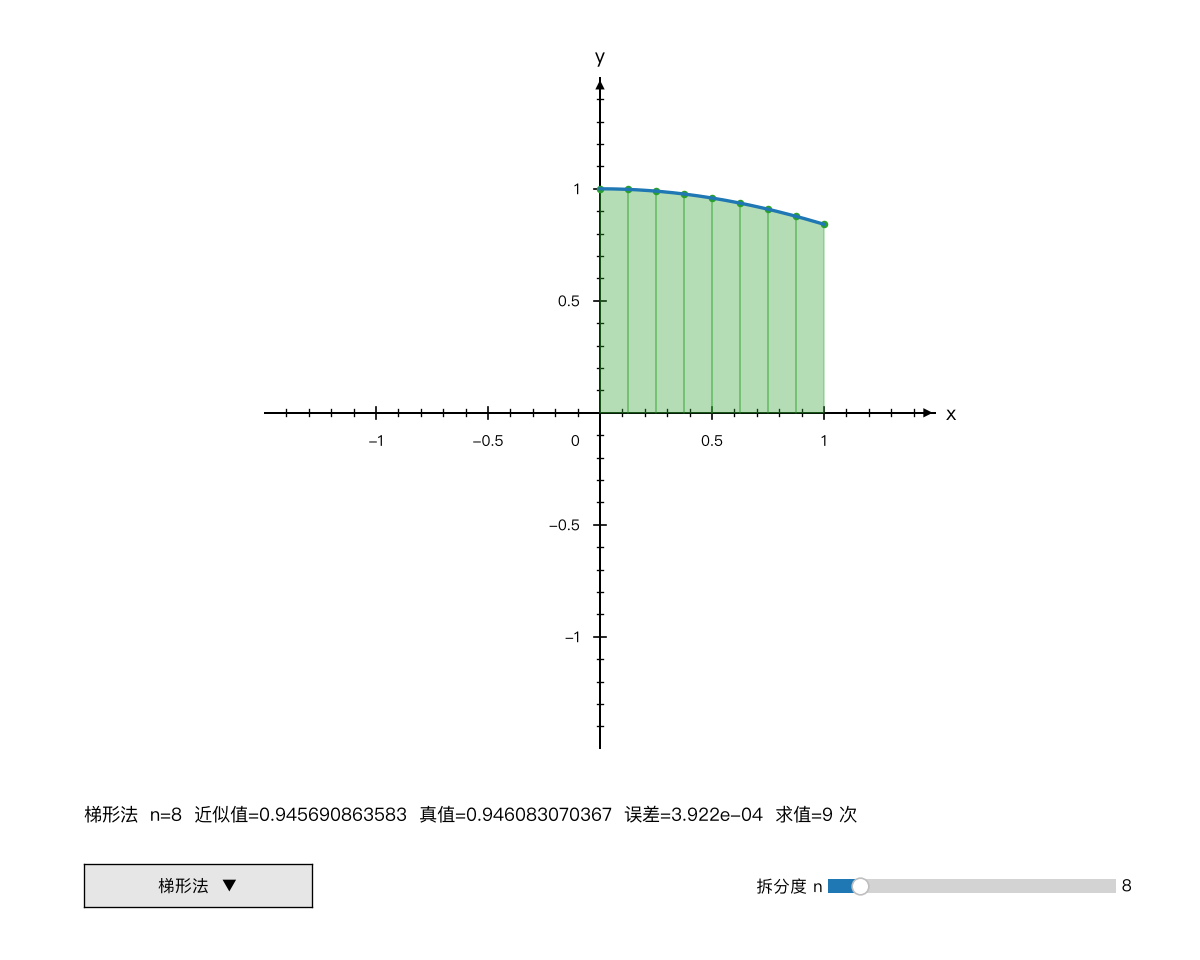
\includegraphics[width=0.48\textwidth]{ui_trapezoid.png}
    \caption{梯形法（$n=8$）：误差 $3.92\times10^{-4}$，9 次求值}
    \label{fig:trapezoid}
\end{figure}

% ---------------------------------------------------------------
\subsection{辛普森法}\label{subsec:simpson}

每相邻两段用过三点的抛物线代替曲线，复化后
\begin{equation}
    S_n=\frac{h}{3}\left[f(a)+4\sum_{k\text{ 奇}}f(a+kh)+2\sum_{k\text{ 偶}}f(a+kh)+f(b)\right],
    \label{eq:simpson}
\end{equation}
其中 $n$ 必须为偶数，误差 $O(h^4)$。奇数下标乘 4、偶数下标乘 2，一个循环完成：
\src{simpson.py}{23}{36}
$n$ 的偶数性由 \code{main.py} 在切换到本方法时把滑块档位改成 $2,4,\dots,64$ 来保证，算法模块不做检查。

运行效果如图 \ref{fig:simpson}，$n=8$ 时 $S_8=0.946083310888$，误差 $2.41\times10^{-7}$，同样 9 次函数求值，比梯形准三个数量级。

\begin{figure}[H]
    \centering
    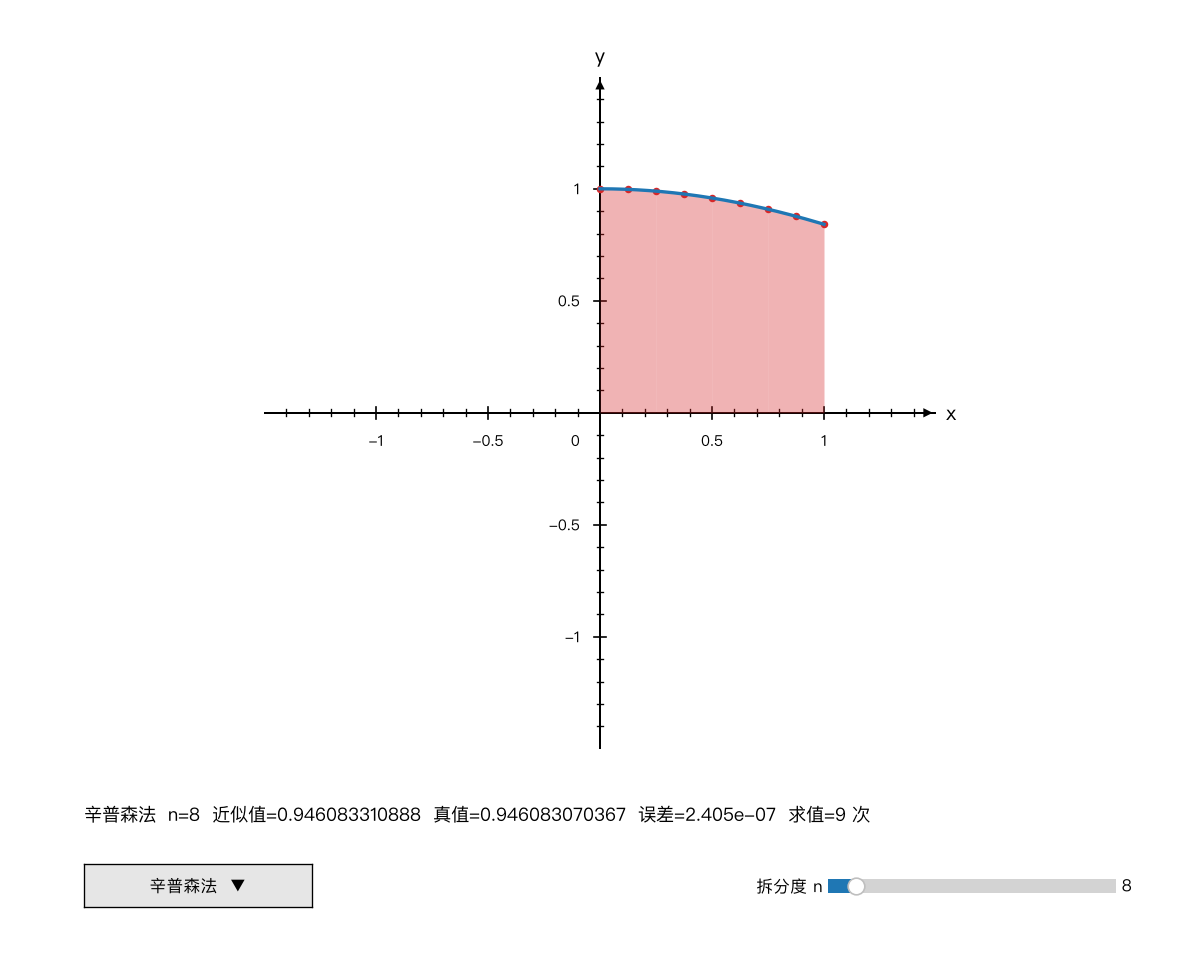
\includegraphics[width=0.48\textwidth]{ui_simpson.png}
    \caption{辛普森法（$n=8$）：误差 $2.41\times10^{-7}$，9 次求值}
    \label{fig:simpson}
\end{figure}

% ---------------------------------------------------------------
\subsection{龙贝格法}\label{subsec:romberg}

复化梯形的误差有展开式 $I-T(h)=c_1h^2+c_2h^4+c_3h^6+\cdots$，只含 $h$ 的偶次幂。
把步长减半得 $I-T(h/2)=c_1h^2/4+c_2h^4/16+\cdots$，两式消去 $c_1h^2$ 项：
\begin{equation}
    I\approx\frac{4T(h/2)-T(h)}{3}.
    \label{eq:extrap}
\end{equation}
这就是 Richardson 外推，误差阶从 $O(h^2)$ 跳到 $O(h^4)$。对一列二分步长的梯形值反复外推，得到龙贝格表
\begin{equation}
    R_{k,0}=T_k,\qquad
    R_{k,j}=R_{k,j-1}+\frac{R_{k,j-1}-R_{k-1,j-1}}{4^j-1},
    \label{eq:romberg}
\end{equation}
对角元 $R_{k,k}$ 的误差为 $O(h^{2k+2})$。

实现分两步。\code{trapezoid\_levels} 从 $T_0$ 出发，每二分一次只在新出现的 $2^{k-1}$ 个中点求值，
用递推 $T_k=\tfrac12T_{k-1}+h_k\sum_{i}f\bigl(a+(2i-1)h_k\bigr)$ 算出整个梯形序列，总共只需 $2^k+1$ 次求值：
\src{romberg.py}{26}{40}
\code{table} 按式 \eqref{eq:romberg} 逐行外推，第 $k$ 行只引用第 $k-1$ 行：
\src{romberg.py}{43}{59}
对本题 $k=3$ 时表中的数值为
\begin{table}[H]
    \centering
    \caption{龙贝格表（$k=3$）：第一列为二分梯形值，向右每列外推一次}
    \label{tab:romberg}
    \begin{tabular}{ccccc}
        \toprule
        $k$ & $T_k$（$2^k$ 段） & 外推 1 次 & 外推 2 次 & 外推 3 次 \\
        \midrule
        0 & 0.920735492 &            &            &            \\
        1 & 0.939793285 & 0.946145882 &            &            \\
        2 & 0.944513522 & 0.946086934 & 0.946083004 &            \\
        3 & 0.945690864 & 0.946083311 & 0.946083069 & 0.946083070 \\
        \bottomrule
    \end{tabular}
\end{table}
每一列都比前一列收敛得快，右下角 $R_{3,3}$ 即最终结果：误差 $2.0\times10^{-11}$，
而最细一层梯形 $T_3$ 本身只有 $3.9\times10^{-4}$，外推没有增加任何函数求值。
界面上画的是最细一层（$2^k$ 段）梯形，报出的是外推值（图 \ref{fig:romberg}）。

\begin{figure}[H]
    \centering
    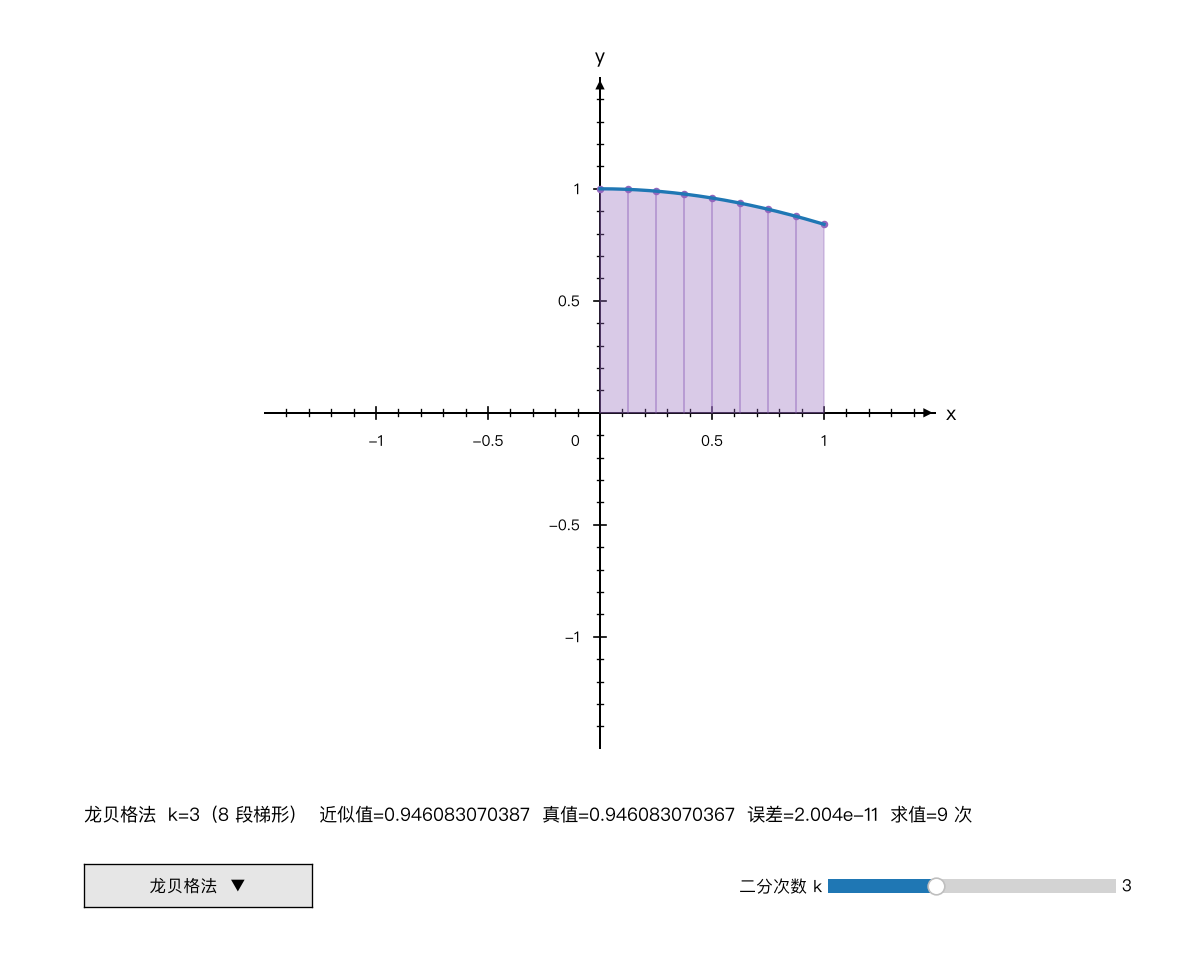
\includegraphics[width=0.48\textwidth]{ui_romberg.png}
    \caption{龙贝格法（$k=3$，8 段梯形）：误差 $2.00\times10^{-11}$，9 次求值}
    \label{fig:romberg}
\end{figure}

% ---------------------------------------------------------------
\subsection{高斯-勒让德法}\label{subsec:gauss}

前面所有方法的节点都固定在等分点上，权重由“对低次多项式精确”确定。
高斯求积把\textbf{节点位置}也作为未知量：$m$ 个节点与权重共 $2m$ 个自由度，
恰好可令 $1,t,\dots,t^{2m-1}$ 共 $2m$ 个多项式积分精确，代数精度 $2m-1$，是 $m$ 个节点所能达到的上限。
满足条件的节点是 $m$ 次勒让德多项式 $P_m(t)$ 的零点，权重 $A_i=2/\bigl[(1-t_i^2)P_m'(t_i)^2\bigr]$，
在标准区间 $[-1,1]$ 上定义，通过线性变换
\begin{equation}
    x=\frac{b-a}{2}\,t+\frac{a+b}{2},
    \qquad
    \int_a^b f(x)\,\mathrm{d}x=\frac{b-a}{2}\sum_{i=1}^{m}A_i\,f(x_i)
    \label{eq:gauss}
\end{equation}
搬到 $[a,b]$。$m=1$ 时节点 $x=(a+b)/2$、权重退化为中矩形；误差 $O(h^{2m})$（以区间长度计）。

节点与权重不手算也不查表，直接调用 \code{np.polynomial.legendre.leggauss(m)}，
它用 Newton 迭代在双精度下求出 $P_m$ 的零点与对应权重：
\src{gauss.py}{24}{33}
\code{gauss\_rule} 按式 \eqref{eq:gauss} 加权求和。注意对每个节点单独调用 \code{f}，而不是把数组整体传入——
\code{function.f} 内部有 \code{x == 0.0} 分支，传 numpy 数组会因真值不唯一而抛 \code{ValueError}：
\src{gauss.py}{46}{58}

运行效果如图 \ref{fig:gauss}，$m=3$ 时得 $0.946083134078$，误差 $6.37\times10^{-8}$，仅 3 次函数求值。
高斯公式没有“分段”概念，界面上在每个节点处画一条竖线到曲线并标点。

\begin{figure}[H]
    \centering
    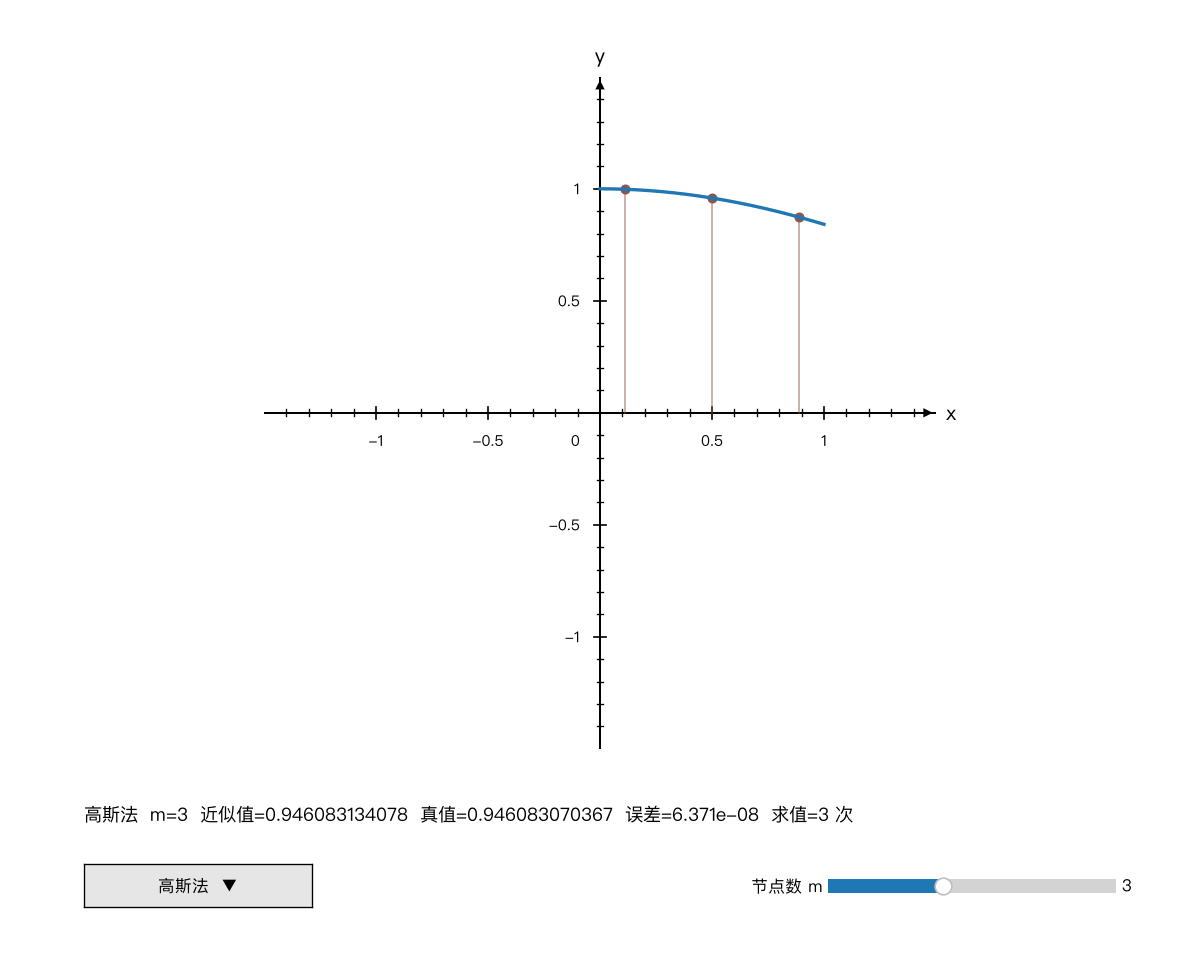
\includegraphics[width=0.48\textwidth]{ui_gauss.png}
    \caption{高斯法（$m=3$）：误差 $6.37\times10^{-8}$，3 次求值}
    \label{fig:gauss}
\end{figure}

% ---------------------------------------------------------------
\subsection{五种方法对比}\label{subsec:compare}

\begin{table}[H]
    \centering
    \caption{五种方法在默认参数下的结果（真值 $I=0.946083070367183\cdots$，误差 $=|I_{\text{近似}}-I|$）}
    \label{tab:compare}
    \begin{tabular}{lcccc}
        \toprule
        方法 & 参数 & 近似值 & 误差 & 求值次数 \\
        \midrule
        矩形法（中） & $n=8$ & 0.946279196286 & $1.96\times10^{-4}$  & 8 \\
        梯形法       & $n=8$ & 0.945690863583 & $3.92\times10^{-4}$  & 9 \\
        辛普森法     & $n=8$ & 0.946083310888 & $2.41\times10^{-7}$  & 9 \\
        龙贝格法     & $k=3$ & 0.946083070387 & $2.00\times10^{-11}$ & 9 \\
        高斯法       & $m=3$ & 0.946083134078 & $6.37\times10^{-8}$  & 3 \\
        \bottomrule
    \end{tabular}
\end{table}

\section{结论}\label{sec:conclusion}

\begin{enumerate}
    \item 五种方法都正确收敛到 $I=0.946083070367183\cdots$，误差与理论阶数一致：
        矩形法与梯形法为 $O(h^2)$，辛普森法为 $O(h^4)$，龙贝格法经 $k$ 次外推可达 $O(h^{2k+2})$，
        高斯法 $m$ 个节点可达代数精度 $2m-1$。
    \item 同样 9 次函数求值，梯形法误差 $3.9\times10^{-4}$，辛普森法 $2.4\times10^{-7}$，龙贝格法 $2.0\times10^{-11}$：
        辛普森法是“换一种拟合”，龙贝格法是“对已有结果做外推”，两者都比单纯加密区间划算得多。
    \item 高斯法用 3 次求值达到 $6.4\times10^{-8}$，是求值次数最少的方法；龙贝格法在同等求值次数下精度最高。
        实际工程中若被积函数求值代价高，优先考虑高斯求积；若已有梯形程序且要求高精度，龙贝格外推是最省事的升级路径。
    \item 交互程序把五种方法放在同一坐标系下实时切换、同屏比较误差与求值次数，
        直观展示了“近似图形—参数—精度”三者的联系。
\end{enumerate}

\appendix
\section{文件清单与运行方式}

\begin{table}[H]
    \centering
    \begin{tabular}{ll}
        \toprule
        文件 & 职责 \\
        \midrule
        \texttt{function.py}   & 被积函数、积分区间、幂级数真值 \\
        \texttt{rectangle.py}  & 矩形法（左/中/右） \\
        \texttt{trapezoid.py}  & 梯形法 \\
        \texttt{simpson.py}    & 辛普森法 \\
        \texttt{romberg.py}    & 龙贝格法（二分梯形 + Richardson 外推） \\
        \texttt{gauss.py}      & 高斯-勒让德法 \\
        \texttt{axes.py}       & 手工绘制的穿过原点的 x/y 数轴 \\
        \texttt{dropdown.py}   & 下拉选择栏控件 \\
        \texttt{main.py}       & 交互程序编排 \\
        \bottomrule
    \end{tabular}
\end{table}

在作业二目录下运行：

\begin{codebox}
\begin{lstlisting}[style=vscode,language={},numbers=none]
$ uv run main.py
\end{lstlisting}
\end{codebox}

\end{document}
